\documentclass{beamer}
\usepackage{tikz}
\usepackage{pgfplots}

\pgfplotsset{compat=1.17}
\usetikzlibrary{patterns,decorations.pathmorphing}
\begin{document}
    % Your presentation content goes 
    % Title frame
    \author{D. Heurtel-Depeiges}
    \title{Oscillateur harmonique et amorti, forçage}
    \date{Novembre 2023}
    \begin{frame}
        \titlepage
    \end{frame}
    % Other frames
    \section*{Oscillateurs libres}
    \begin{frame}{Oscillateur libre non amorti}
        \begin{block}{Equation différentielle}
            \begin{equation}
                \ddot{x} + \omega_0^2 x = 0
            \end{equation}
        \end{block}
        \begin{block}{Solution}
            \begin{equation}
                x(t) = A \cos(\omega_0 t + \varphi)
            \end{equation}
        \end{block}
        \begin{block}{Exemple}
            % Tikz picture of a spring/mass system
            \begin{center}
            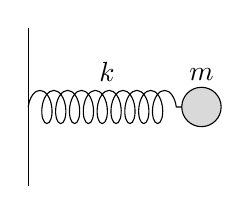
\begin{tikzpicture}[>=latex]

              % Wall
              \draw (0,0) -- (0,2);
            
              % Spring
              \draw [decorate,decoration={coil,amplitude=6pt,segment length=5pt}] (0,1) -- (2,1);
              \draw (2,1) -- (2.2,1);
              \draw (0,1) -- (0,1.5);
            
              % Mass
              \draw [fill=gray!30] (2.2,1) circle (0.25) node[above=6pt] {$m$};
            
              % Ground
              %\draw (2,1.5) -- (6,1.5);
            
              % Spring Constant
              \node[above] at (1,1.2) {$k$};
        
        \end{tikzpicture}
        \end{center}
        Dans cet exemple, (en ignorant les forces selon l'axe $x$), on obtient l'équation différentielle suivante:
        \begin{equation}
            m \ddot{x} = -k x \iff \ddot{x} + \frac{k}{m} x = 0
        \end{equation}
        On introduit naturellement $w_0^2 = \frac{k}{m}$. Puis on résout l'équation différentielle à l'aide des conditions initiales...
        \end{block}
    \end{frame}
\section{Oscillateur libre}
    \begin{frame}{Oscillateur libre amorti}
        % Start with a tikz picture of a spring/mass system with a damper
        \begin{center}
            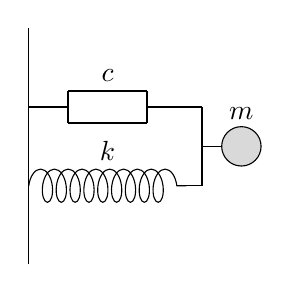
\begin{tikzpicture}[>=latex]

                % Wall
                \draw (0,0) -- (0,3);
            
                % Spring
                \draw [decorate,decoration={coil,amplitude=6pt,segment length=5pt}] (0,1) -- (2,1);
                \draw (2,1) -- (2.2,1);
                % Damper 
                \draw [thick] (0,2) -- (0.5,2);
                \draw [thick] (0.5,1.8) -- (0.5,2.2);
                \draw [thick] (0.5,1.8) -- (1.5,1.8);
                \draw [thick] (0.5,2.2) -- (1.5,2.2);
                \draw [thick] (1.5,1.8) -- (1.5,2.2);
                \draw [thick] (1.5,2) -- (2.2,2);

                %Join the damper and spring
                \draw (2.2,2) -- (2.2,1);

                % Mass
                \draw [fill=gray!30] (2.7,1.5) circle (0.25) node[above=6pt] {$m$};
                % Join the mass to the vertical bar
                \draw (2.45,1.5) -- (2.2,1.5);
                % Spring Constant
                \node[above] at (1,1.2) {$k$};
                % Damping Constant
                \node[above] at (1,2.2) {$c$};

            \end{tikzpicture}
        \end{center}
        
        \begin{block}{Equation différentielle}
            \begin{equation}
                m \ddot{x} + c \dot{x} + k x = 0
            \end{equation}
            Ce qui se réécrit:
            \begin{equation}
                \ddot{x} + 2\lambda \dot{x} + \omega_0^2 x = 0
            \end{equation}
            $\implies$ On vérifie tout le temps que $\tau = \frac{1}{\lambda}$ est bien homogène à un temps et $\omega_0$ à une pulsation (donc fréquence $\propto T^{-1}$)
        \end{block}
    \end{frame}
    \begin{frame}
        On sait la forme que va prendre les solutions de cette équation différentielle (ça se démontre). 
        \textbf{Idée générale}, on va chercher les solutions sous la forme $x(t) = A e^{rt}$, où $r$ est un nombre complexe. On obtient alors l'équation caractéristique suivante:
        \begin{equation}
            r^2 + 2\lambda r + \omega_0^2 = 0
        \end{equation}
        Déterminons les solutions de cette équation caractéristique. Soit $\Delta = 4\lambda^2 - 4\omega_0^2 = 4(\lambda^2 - \omega_0^2)$. On a alors trois cas possibles:\begin{itemize}
            \item $\Delta > 0 \iff Q = \frac{w_0}{2\lambda} < 1/2$ (régime apériodique) $\implies$ deux solutions réelles $r_1$ et $r_2$.
            \item $\Delta = 0 \iff Q = \frac{w_0}{2\lambda} = 1/2$ (régime critique) $\implies$ une solution double $r_1 = r_2$ réelle.
            \item $\Delta < 0 \iff Q = \frac{w_0}{2\lambda} > 1/2$ (régime pseudo-périodique) $\implies$ deux solutions complexes conjuguées $r_1 = -\lambda + i \beta$ et $r_2 = -\lambda - i \beta$.
        \end{itemize}
    \end{frame}
    \begin{frame}{Deux solutions réelles}
        \begin{block}{Solution générale}
            \begin{equation}
                x(t) = A e^{r_1 t} + B e^{r_2 t}
            \end{equation}
        \end{block}
        On peut décompser ça en cosinus et sinus hyperboliques...mais c'est pas très utile.
        \begin{block}{Allure de la soultion}
            % Draw an exponential function to 0
            \begin{tikzpicture}
                \begin{axis}[
                  width=8cm,
                  height=6cm,
                  xlabel={$t$},
                  ylabel={$x(t)$},
                  domain=0:10,
                  samples=100,
                  axis lines=middle,
                  enlargelimits=upper,
                  legend style={at={(0.5,-0.15)},anchor=north},
                ]
              
                \addplot[blue,thick] {exp(-0.5*x) + 1/2*exp(-2*x)};
                
                \end{axis}
              \end{tikzpicture}
        \end{block}
    \end{frame}

    \begin{frame}{Deux solutions complexes}
        \begin{block}{Solution générale}
            \begin{equation}
                x(t) = e^{-\lambda t} \left(A \cos(\beta t) + B \sin(\beta t)\right)
            \end{equation}
            En général on réécrit $\beta = \omega$ (attention pas $\omega_0$).
        \end{block}
        \begin{block}{Allure de la solution}
            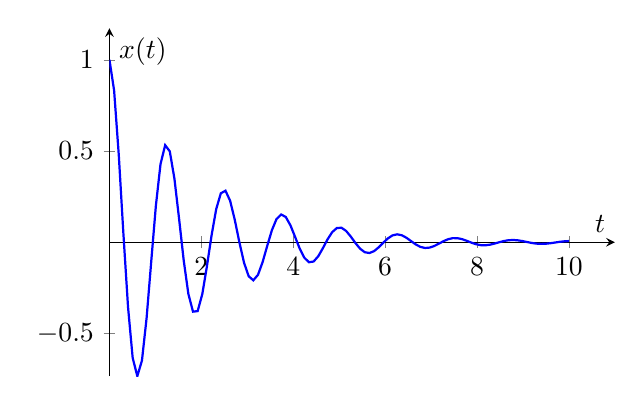
\begin{tikzpicture}
                \begin{axis}[
                  width=8cm,
                  height=6cm,
                  xlabel={$t$},
                  ylabel={$x(t)$},
                  domain=0:10,
                  samples=100,
                  axis lines=middle,
                  enlargelimits=upper,
                  legend style={at={(0.5,-0.15)},anchor=north},
                ]
              
                \addplot[blue,thick] {exp(-0.5*x)*cos(deg(5*x))};
                
                \end{axis}
              \end{tikzpicture}
        \end{block}
    \end{frame}
       \begin{frame}{Quelques éléments en plus (sur les régimes apériodique et pseudo-périodique)}
        \begin{itemize}
            \item Décrément logarithmique (pseudo-périodique)$\delta = \ln \left(\frac{x(t)}{x(t+T)}\right) = \lambda T$
            Or $T=\frac{2\pi}{\omega}$, donc $\delta = \frac{2\pi}{\omega} \lambda = \frac{2\lambda\pi}{\omega_0} \frac{\omega_0}{\omega} = \frac{\pi}{Q}\frac{\omega_0}{\omega}$
            \item Plus le facteur de qualité est grand, plus le système est proche d'un oscillateur harmonique $\omega\approx \omega_0$ et $\delta\ll 1$.
            \item Plus le facteur de qualité est petit, plus le système est proche d'un régime apériodique totalement amorti (on ne peut plus parler de pulsation ni de décrément logarithmique).
        \end{itemize}
    \end{frame}
    \begin{frame}{Cas particulier : une unique solution réelle}
        Si $Q = 1/2$, on a une solution double $r_1 = r_2 = -\lambda$. On peut alors écrire la solution sous la forme (à connaître):
        \begin{equation}
            x(t) = e^{-\lambda t} \left(A + B t\right)
        \end{equation}
        Comme pour toutes les équations précédentes, on peut déterminer $A$ et $B$ à l'aide des conditions initiales.

        $\implies$ On peut montrer que le régime critique est le plus rapide pour revenir à l'équilibre (sans dépasser l'équilibre).
    \end{frame}

\section*{Oscillateur forcé}
\begin{frame}{Oscillateur forcé}
    \begin{block}{Equation différentielle}
        \begin{equation}
            \ddot{x} + 2\lambda \dot{x} + \omega_0^2 x = F_0 \cos(\omega t)
        \end{equation}
    \end{block}
    \begin{block}{Solution générale}
        Quelles que soient les conditions initiales, on peut écrire la solution générale comme une solution particulière du cas libre + une solution du cas libre stationnaire (autrement dit une solution qui n'évolue plus dans sa nature).

        On s'intéresse donc à la solution du cas forcé stationnaire. 
    \end{block}
    
\end{frame}
\begin{frame}{Solution du cas forcé, l'idée}

        On cherche une solution qui a la même pulsation que celle du forçage. On pose donc $x(t) = A \cos(\omega t + \varphi)$.

        On a donc $x(t) = \mathfrak{R}(A\exp(i(\omega t+\varphi)))$. On a les parties réelles qui collent...pourquoi pas ne pas imposer que les parties imaginaires aussi. 

        On écrit donc $\underline{x(t)} = A \exp(i(\omega t + \varphi))$. On a alors:\begin{align}
             \underline{\ddot{x(t)}} &= -\omega^2 \underline{x(t)} \\
            \underline{\dot{x(t)}} &= i\omega \underline{x(t)}
        \end{align}

        On obtient donc l'équation suivante:
        \begin{equation}
            -\omega^2 \underline{x(t)} + 2\lambda i \omega \underline{x(t)} + \omega_0^2 \underline{x(t)} = F_0 e^{i\omega t}
        \end{equation}
    
\end{frame}

\begin{frame}
    On peut simplifier cette équation en divisant par $\exp(i\omega t)$, on obtient alors:
    \begin{equation}
        -\omega^2 \underline{x_0} + 2\lambda i \omega \underline{x_0} + \omega_0^2 \underline{x_0} = F_0
    \end{equation}
    Avec $\underline{x_0} = A e^{i\varphi}$.

    Ce qui se réécrit:
    \begin{equation}
        \underline{x_0} = \frac{F_0}{\omega_0^2 - \omega^2 + 2i\lambda \omega}
    \end{equation}
    On obtient $A$ et un "représentant" de $\varphi$ (modulo $2\pi$) en considérant respectivement le module de la fraction et son argument.

    $\implies$ Cas de base des filtres linéaires (que tu verras sûrement plus tard).
\end{frame}

\end{document}
